\documentclass{article}
\usepackage[a4paper, margin=1cm]{geometry}
\usepackage{tabularx}
\usepackage{graphicx}
\usepackage{wrapfig}
\usepackage{amsmath}
\usepackage{listings}
\usepackage{xcolor}

\lstset{
  language=C++,
  basicstyle=\ttfamily\small,
  keywordstyle=\color{blue}\bfseries,
  commentstyle=\color{gray},
  stringstyle=\color{red},
  showstringspaces=false,
  numbers=left,
  numberstyle=\tiny\color{gray},
  frame=single,
  breaklines=true,
  tabsize=2
}


\title{\textbf{LAPORAN TUGAS 3}}
\author{Race Recognition Rush}
\date{}

\begin{document}

\maketitle
\begin{center}
    
\includegraphics[scale=0.4]{logo-ukdw.png}
\end{center}

\begin{table}[h]
    \centering
    \renewcommand{\arraystretch}{1.5}
    \begin{tabularx}{\textwidth}{|c|X|}
        \hline
        Mata kuliah	& TI0263 – Kecerdasan Buatan (GRUP C) \\
        \hline
        Dosen Pengampu & Gloria Virginia, S.Kom., MAI., Ph.D \\
        \hline
        Nama Kelompok & C8 \\
        \hline 
        Anggota Kelompok & 
        \begin{minipage}{\textwidth}
            \vspace{5px}
            \begin{enumerate}
                \item 71230985 - Tomas Becket
                \item 71231002 – Philip Deric Kho  
                \item 71231015 - Karel Marley Bala Bakior
                \item 71231017 - Paulus Ungirwalu
                \item 71231061 - Syendhi Reswara. S
            \end{enumerate}
            \vspace{5px}
        \end{minipage} \\
        \hline
        Deklarasi & Dengan ini kami menyatakan bahwa tugas ini merupakan hasil karya kelompok kami, tidak ada manipulasi data serta bukan merupakan plagiasi dari karya orang lain. \\
        \hline
    \end{tabularx}
\end{table}


\vfill

\noindent
\makebox[0pt][l]{%
  \begin{tabular}{@{}c@{}}
  
\includegraphics[scale=0.2]{fti-ukdw.png}
  \end{tabular}%
}\hfill
\textbf{\begin{tabular}{@{}c@{}}
    \textbf{UNIVERSITAS KRISTEN DUTA WACANA} \\
Fakultas Teknologi Informasi \\ 
Program Studi Informatika \\ 
  \end{tabular}%
}\hfill
\makebox[0pt][r]{%
  \begin{tabular}{@{}c@{}}
  
\includegraphics[scale=0.133]{tiukdw.jpg}
  \end{tabular}%
}

\break

\section*{Tugas3}
\subsection{
\text{Jelaskan 1 metode yang digunakan sebagai mesin inferensi aplikasi PAM
kelompok Anda!}}
% \newline


Aplikasi kami akan mengatahui ras dari wajah pengguna (Jawa, Cina, Papua) menggunakan face recognition berbasis knowledge based dengan aturan-aturan yang telah ditentukan.
Berdasarkan data tersebut, program kami akan menentukan lokasi pada peta UKDW yang mana memiliki orang-orang dengan ras yang sama.
Setelah lokasi ditentukan, sistem akan menggunakan algoritma \boxed{A*} atau \boxed{Dijkstra} untuk menghitung dan menetukan rute tercepat menuju lokasi tersebut.
\newline

\noindent Contoh:

Pengguna akan diidentifikasi pada aplikasi dan ternyata memiliki ras China melalui face recognition. Sistem menggunakan metode forward chaining untuk mencocokkan hasil ini dengan aturan:
\newline
Jika ras = China, maka tujuan = Gedung Agape (jika gedung tersebut memiliki persentase ras China tertinggi)
\newline
Setelah itu, sistem mengambil lokasi pengguna saat ini (misalnya di Kantin UKDW) dan menghitung rute tercepat ke Gedung Agape  menggunakan algoritma A* atau Dijkstra. sehingga hasil akhirnya pengguna akan ditampilkan peta UKDW dengan jalur optimal menuju Gedung Agape, tempat di mana kemungkinan besar ada orang dengan ras yang sama.

\subsection{Contoh kasus}

There are $n$ cities and $m$ flight connections between them. Your task is to determine the length of the shortest route from \textbf{Syrjälä} to every city.

\subsection*{Input}

The first input line has two integers $n$ and $m$: the number of cities and flight connections. The cities are numbered $1,2,\dots,n$, and city $1$ is \textbf{Syrjälä}.
After that, there are $m$ lines describing the flight connections. Each line has three integers $a$, $b$ and $c$: a flight begins at city $a$, ends at city $b$, and its length is $c$. Each flight is a one-way flight.

You can assume that it is possible to travel from Syrjälä to all other cities.

\subsection*{Output}

Print $n$ integers: the shortest route lengths from Syrjälä to cities $1,2,\dots,n$.

\subsection*{Constraints}
\begin{itemize}
    \item $1 \le n \le 10^5$
    \item $1 \le m \le 2 \cdot 10^5$
    \item $1 \le a,b \le n$
    \item $1 \le c \le 10^9$
\end{itemize}

\vfill

\noindent
\makebox[0pt][l]{%
  \begin{tabular}{@{}c@{}}
  
\includegraphics[scale=0.2]{fti-ukdw.png}
  \end{tabular}%
}\hfill
\textbf{\begin{tabular}{@{}c@{}}
    \textbf{UNIVERSITAS KRISTEN DUTA WACANA} \\
Fakultas Teknologi Informasi \\ 
Program Studi Informatika \\ 
  \end{tabular}%
}\hfill
\makebox[0pt][r]{%
  \begin{tabular}{@{}c@{}}
  
\includegraphics[scale=0.133]{tiukdw.jpg}
  \end{tabular}%
}

\subsection*{Example}

\begin{minipage}{0.5\textwidth}
\textbf{Input:}
\begin{verbatim}
3 4
1 2 6
1 3 2
3 2 3
\end{verbatim}

\textbf{Output:}
\begin{verbatim}
0 5 2
\end{verbatim}
\end{minipage}%
\hfill
\begin{minipage}{0.45\textwidth}
\centering
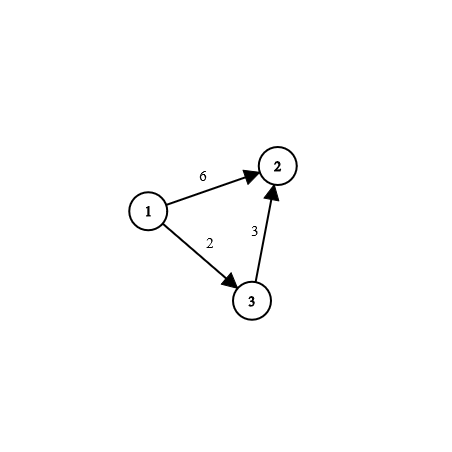
\includegraphics[width=\linewidth]{graph.png}
\end{minipage}

\begin{lstlisting}
#include <bits/stdc++.h>
using ll = long long;
using ull = unsigned long long;
using namespace std;

void solve() {
    int n, m;
    cin >> n >> m;
    
    vector< vector<pair<int, int>> > neighbours(n+1);

    for (int i = 1; i <= m; i++) {
        int city;
        pair<int, int> flight;
        cin >> city >> flight.first >> flight.second;
        neighbours[city].push_back(flight);
    }

    vector<ll> ans(n+1, LONG_LONG_MAX);  // ans untuk answer
    ans[1] = 0;

    using apa_ini = pair<ll, int>; // saya bingung C++ template; oke sip;
    priority_queue<apa_ini, vector<apa_ini>, greater<apa_ini>> pq;
    pq.push({0, 1});

    while (!pq.empty()) {
        auto [distance, target] = pq.top(); pq.pop();
        if (distance > ans[target]) continue; // menghindari pemrosesan input yang memiliki jarak lebih jauh

        for (int i = 0; i < neighbours[target].size(); i++) {
            int t2 = neighbours[target][i].first; 
            ll d2 = neighbours[target][i].second + distance; 

            ll flag = ans[t2];
            ans[t2] = min(ans[t2], d2);

            if (ans[t2] != flag) {
                pq.push({ans[t2], t2});
            }
        }
    }

    for (int i = 1; i <= n; i++) {
        cout << ans[i] << " ";
    } cout << '\n';
}
\end{lstlisting}

\end{document}